\clearpage

\section{Results}

In this section we provide the results of the inclusive and targeted searches. 
The observed and predicted \MET\ distributions for the inclusive analysis are indicated in Fig.~\ref{fig:results_incl}. 
A summary of the results in the signal regions is provided in Table~\ref{tab:results_incl}. 
Good agreement is observed between the data and the predicted background over the full \MET\ range.
The separate results for the ee and $\mu\mu$ channels are presented in App.~\ref{app:results}.

\begin{figure}[!h]
\begin{center}
\begin{tabular}{cc}
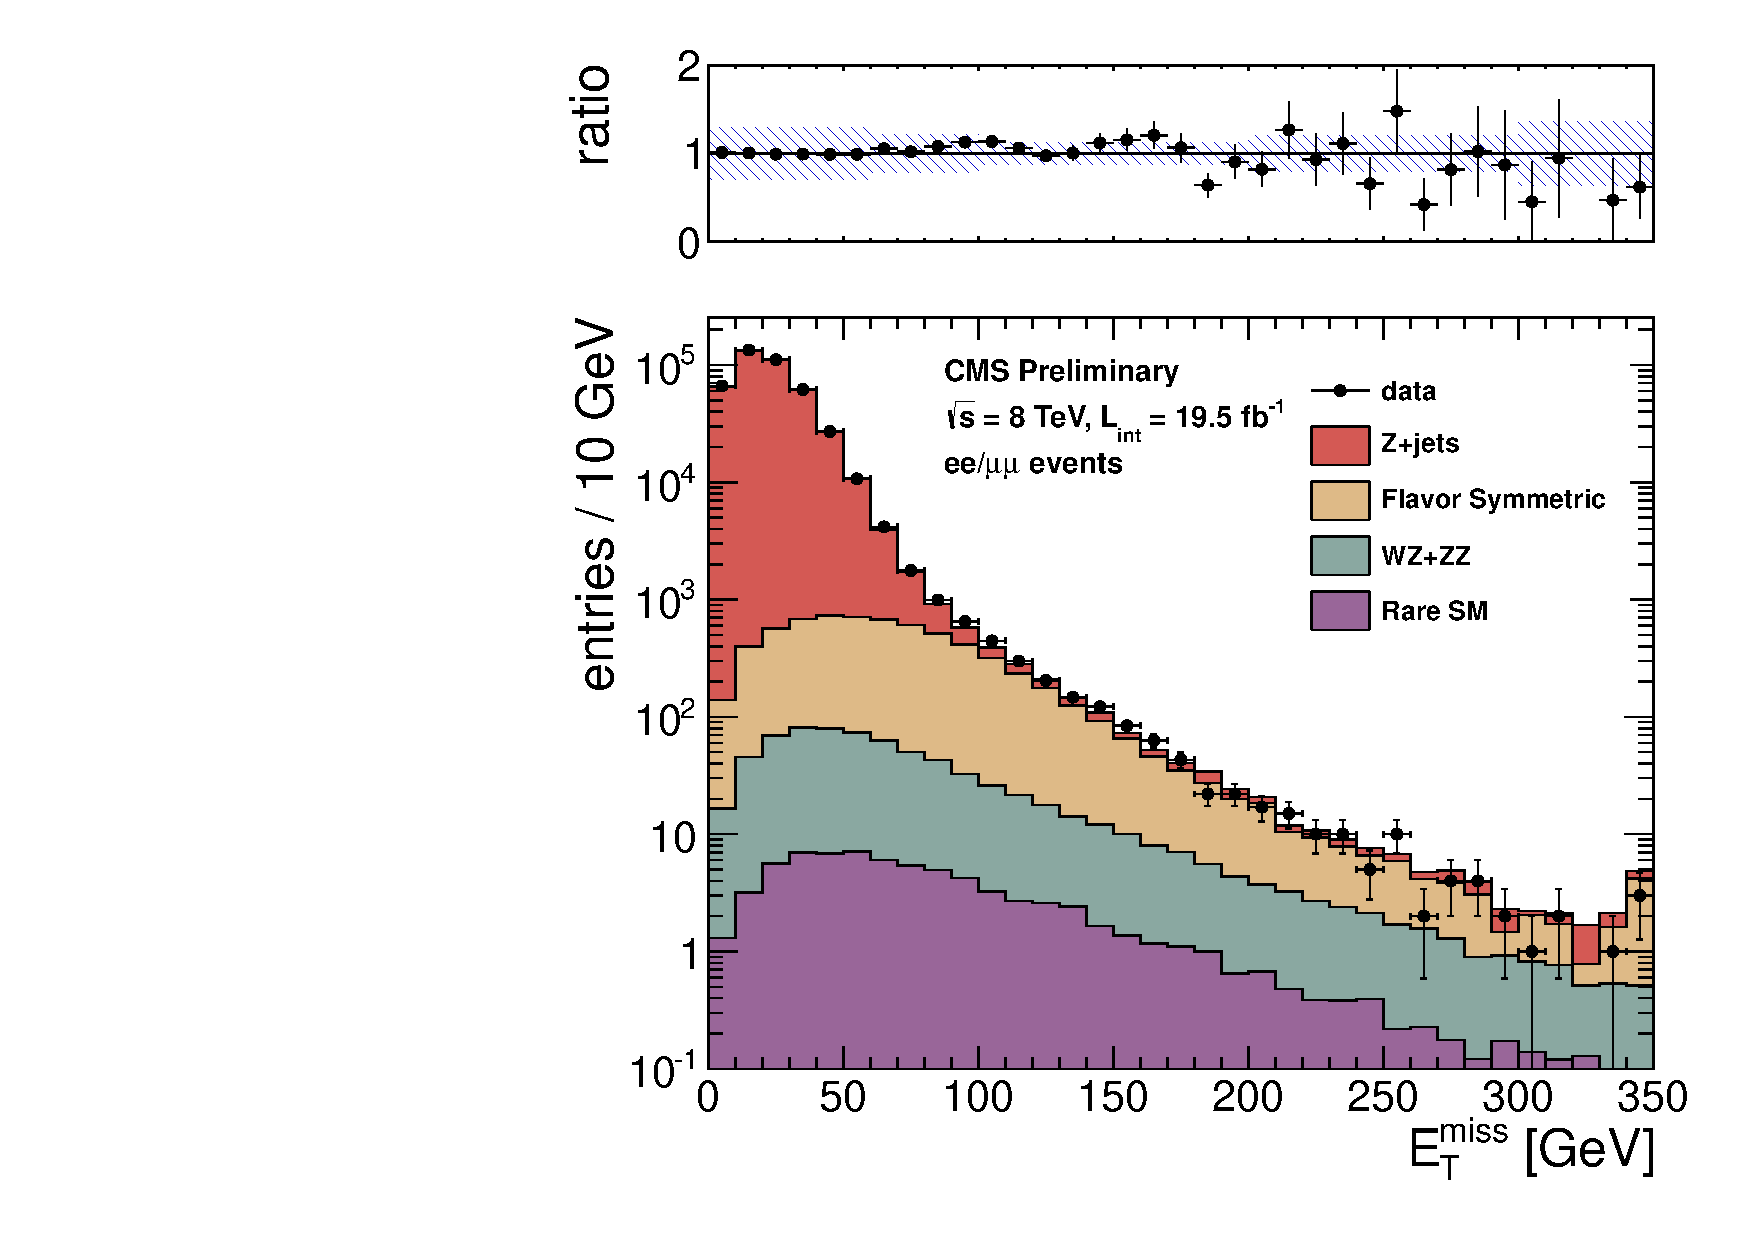
\includegraphics[width=0.6\textwidth]{plots/pfmet_all_19p5fb.pdf}
\end{tabular}
\caption{Results of the inclusive analysis. The observed \MET\ distribution (black points) is compared with the sum of the predicted \MET\
distributions from \zjets, flavor-symmetric backgrounds, and WZ+ZZ backgrounds. The ratio of observed to predicted yields in each bin is
indicated. The error bars indicate the statistical uncertainty in the data and the shaded band indicates the total background uncertainty.
\label{fig:results_incl}
}
\end{center}
\end{figure}



\begin{table}[htb]
\begin{center}
\footnotesize
\caption{\label{tab:results_incl} Summary of results in the inclusive analysis. The total background is the sum of the \zjets\ background predicted from
the \MET\ templates method (\zjets\ bkg), the flavor-symmetric background predicted from e$\mu$ events (FS bkg), and the WZ and ZZ backgrounds predicted from MC
(WZ bkg and ZZ bkg). All uncertainties include both the statistical and systematic components. The Gaussian significance of the deviation between the data 
and total background is indicated for signal regions with at least 20 observed events. }
\begin{tabular}{l|c|c|c|c|c|c}


%Using pfmet out-of-the-box
%DON'T Apply mjj cut in templates
%WZ/ZZ selection : ((((((leptype==0 && (ee==1 || isdata==0))||(leptype==1 && (mm==1 || isdata==0)))&&(ngennu>0))&&(csc==0 && hbhe==1 && hcallaser==1 && ecaltp==1 && trkfail==1 && eebadsc==1 && hbhenew==1))&&(dilmass>81 && dilmass<101))&&(njets>=2))&&(lep1.pt()>20.0 && lep2.pt()>20.0)
%WZ/ZZ weight    : weight * 19.5 * vtxweight * trgeff
%Opening ../output/V00-02-13/babylooper_data_53X_2012ALL_PhotonStitchedTemplate_pfmet.root
%B-veto?   0
%K         0.14
%ee+mm channels: scale em yield by 0.97
%Yields in 0-60 GeV region
%data   : 410573
%gjets  : 414439
%OF     : 2861.58
%WZ     : 295.321
%ZZ     : 38.722
%Rare   : 31.0719
%Scaling gjets by : 0.982887
%SF events 419687
%OF events 43832

%ee/#mu#mu events

\hline
\hline

                      &   \MET\ 0--30 GeV   &  \MET\ 30--60 GeV   & \MET\ 60--100 GeV   &\MET\ 100--200 GeV   &\MET\ 200--300 GeV   & \MET\ $>$ 300 GeV  \\
\hline
        \zjets\ bkg   &309185 $\pm$ 92757   & 98161 $\pm$ 29449   &   4971 $\pm$ 1492   &      222 $\pm$ 67   &    11.3 $\pm$ 3.5   &     2.6 $\pm$ 1.0  \\
             FS bkg   &     972 $\pm$ 151   &    1889 $\pm$ 293   &    2022 $\pm$ 314   &    1011 $\pm$ 157   &   50.7 $\pm$ 15.0   &     7.2 $\pm$ 4.3  \\
             WZ bkg   &  108.9 $\pm$ 54.5   &  186.4 $\pm$ 93.2   &  137.7 $\pm$ 68.9   &   78.7 $\pm$ 39.3   &    11.1 $\pm$ 5.6   &     3.1 $\pm$ 3.1  \\
             ZZ bkg   &    12.1 $\pm$ 6.1   &   26.6 $\pm$ 13.3   &   29.8 $\pm$ 14.9   &   29.8 $\pm$ 14.9   &     6.2 $\pm$ 3.1   &     2.0 $\pm$ 2.0  \\
        rare SM bkg   &    10.1 $\pm$ 5.1   &   21.0 $\pm$ 10.5   &   20.6 $\pm$ 10.3   &    17.9 $\pm$ 9.0   &     3.2 $\pm$ 1.6   &     1.1 $\pm$ 1.1  \\
\hline
          total bkg   &310289 $\pm$ 92757   &100284 $\pm$ 29451   &   7180 $\pm$ 1526   &    1360 $\pm$ 176   &   82.5 $\pm$ 16.8   &    16.0 $\pm$ 5.8  \\
               data   &            311030   &             99543   &              7578   &              1450   &                79   &                 7  \\
%       significance   &       0.0$\sigma$   &      -0.0$\sigma$   &       0.3$\sigma$   &       0.5$\sigma$   &      -0.2$\sigma$   &      -1.4$\sigma$  \\
\hline
\hline


%float Zbkg_yield[nbins]    = { 222.4 , 11.3 ,     2.6  };
%float Zbkg_err[nbins]      = { 67.3 ,  3.5 ,     1.0  };
%float OFbkg_yield[nbins]   = { 1011.4 , 50.7 ,     7.2  };
%float OFbkg_err[nbins]     = { 157.2 , 15.0 ,     4.3  };
%float WZbkg_yield[nbins]   = { 78.7 , 11.1 ,     3.1  };
%float WZbkg_err[nbins]     = { 39.3 ,  5.6 ,     3.1  };
%float ZZbkg_yield[nbins]   = { 29.8 ,  6.2 ,     2.0  };
%float ZZbkg_err[nbins]     = { 14.9 ,  3.1 ,     2.0  };
%float rarebkg_yield[nbins] = { 17.9 ,  3.2 ,     1.1  };
%float rarebkg_err[nbins]   = {  9.0 ,  1.6 ,     1.1  };
%int   data_yield[nbins]    = { 1450 ,   79 ,       7  };



\end{tabular}
\end{center}
\end{table}

\clearpage

The observed and predicted \MET\ distributions for the targeted analysis are indicated in Fig.~\ref{fig:results_targ}. 
The dilepton mass distribution in data is also presented. In this plot, the \zjets\ dilepton mass shape is taken from MC
and normalized to match the data-driven prediction in the dilepton mass window 81--101~GeV. The flavor-symmetric background
is estimated from e$\mu$ events, and the WZ, ZZ, and rare backgrounds are from MC.
A summary of the results in the signal regions is provided in Table~\ref{tab:results_targ}. 
Good agreement is observed between the data and the predicted background over the full \MET\ range.
The separate results for the ee and $\mu\mu$ channels are presented in App.~\ref{app:results}.

\begin{figure}[!h]
\begin{center}
\begin{tabular}{cc}
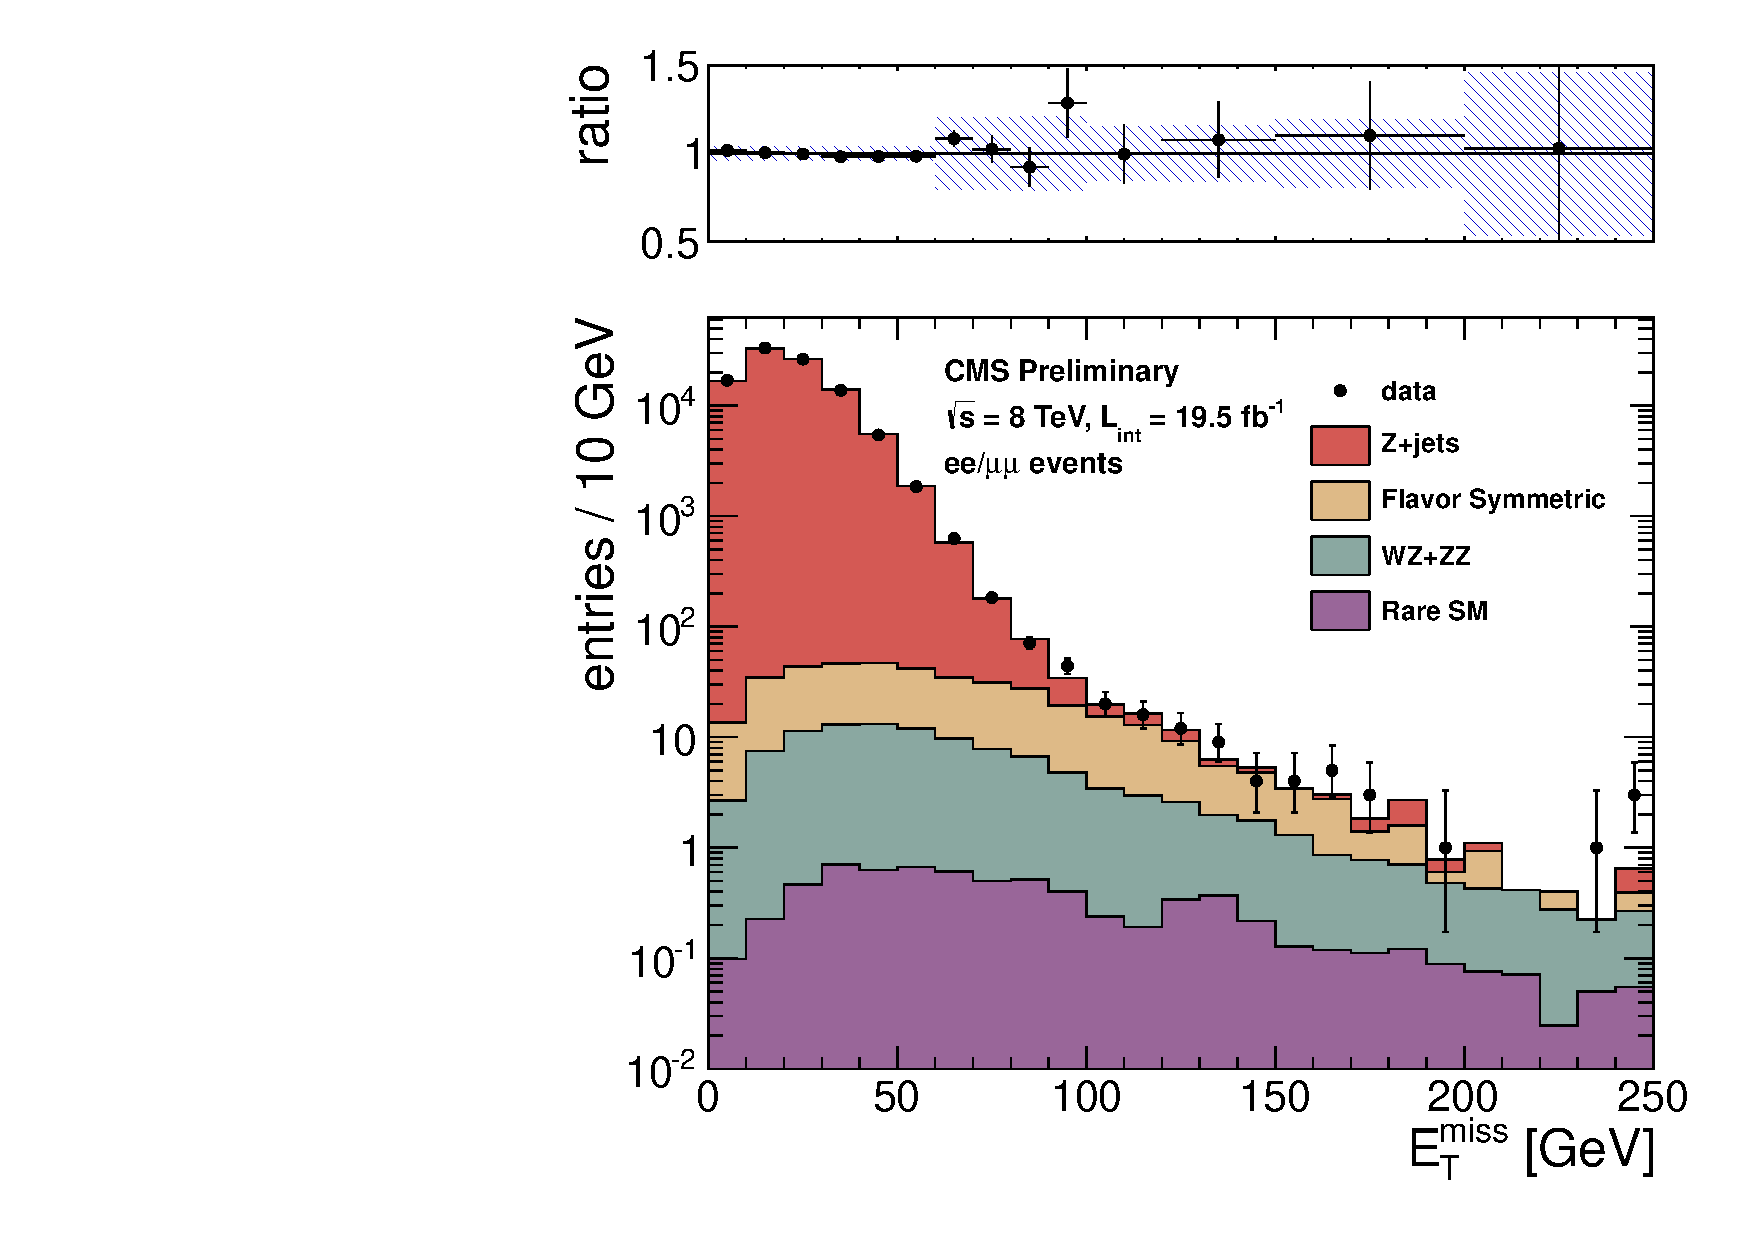
\includegraphics[width=0.49\textwidth]{plots/ZDIJET_metDistribution.pdf} %
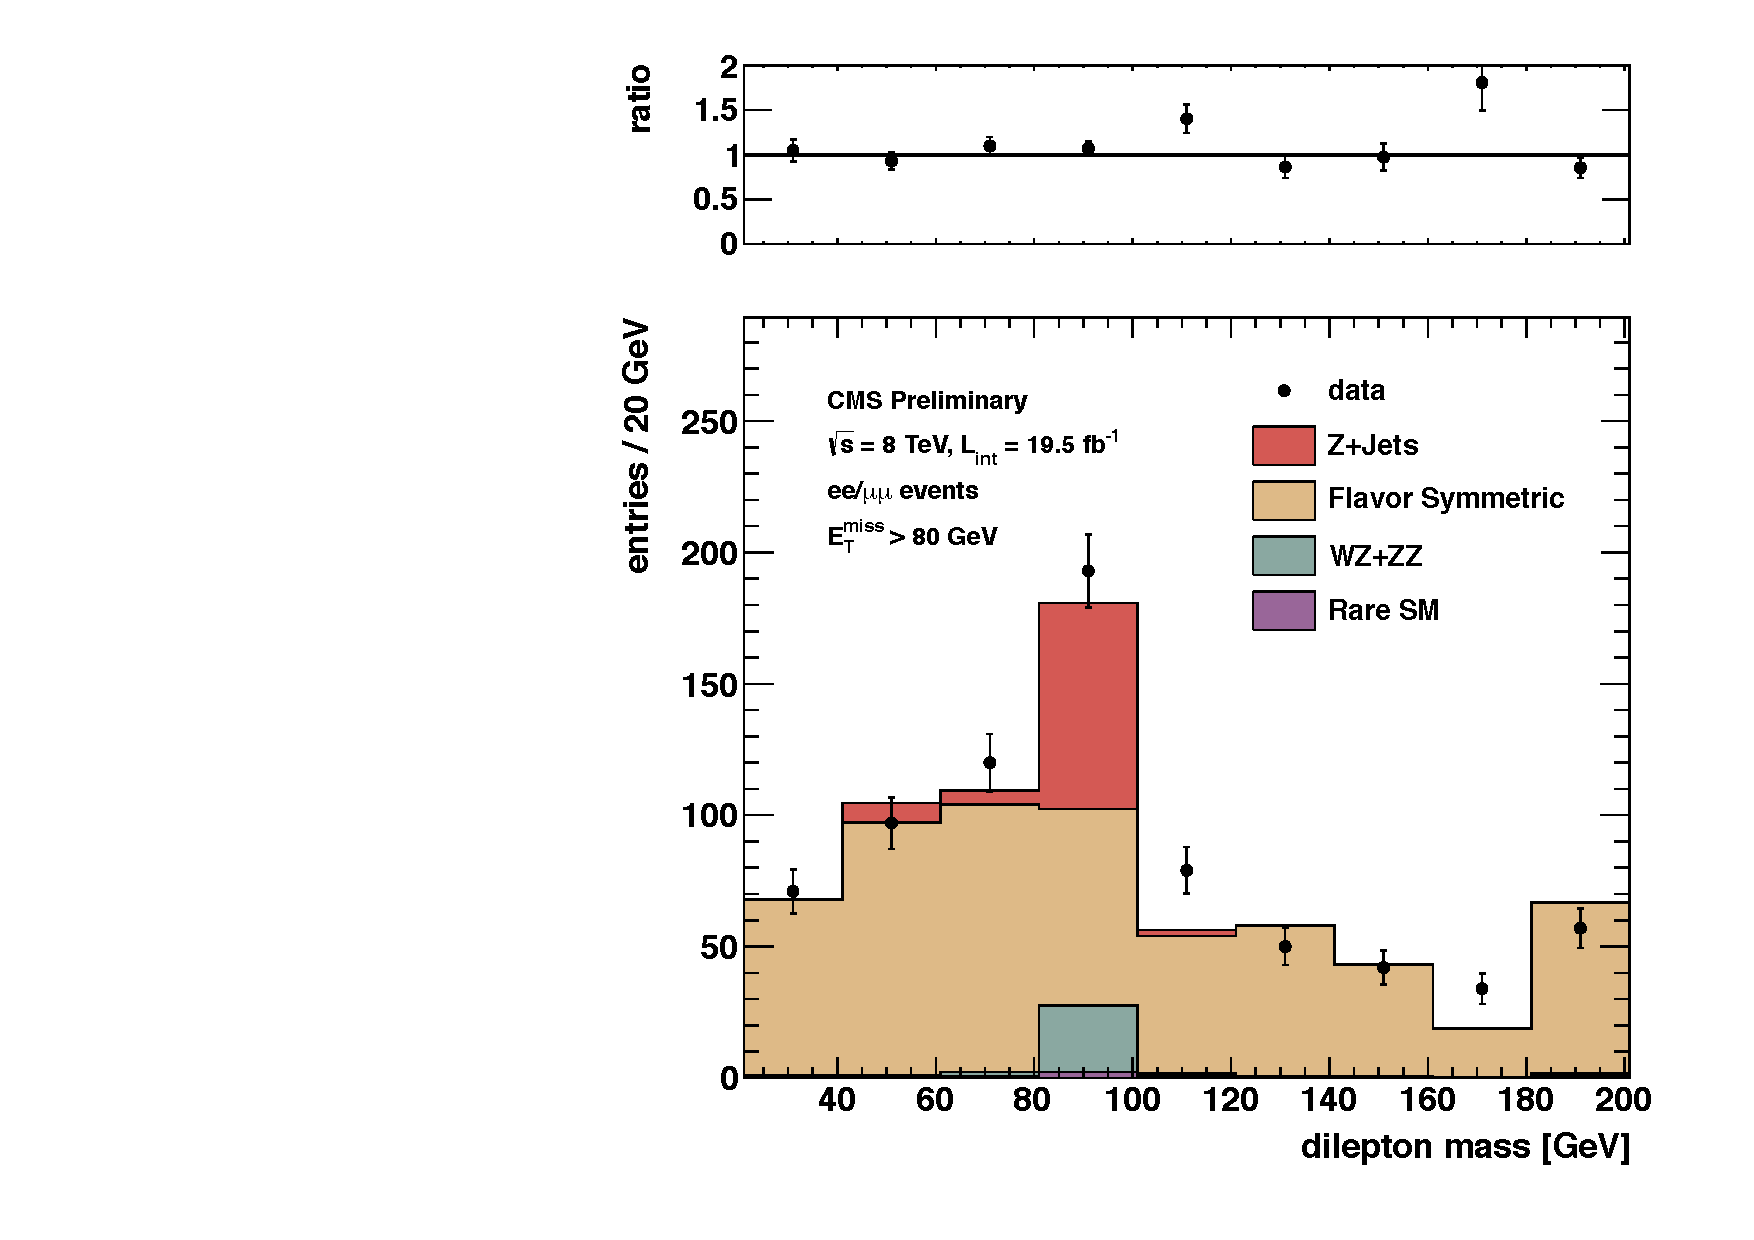
\includegraphics[width=0.49\textwidth]{plots/ZDIJET_mllDistribution.pdf}
\end{tabular}
\caption{The \MET\ distribution after the dilepton mass requirement (left) and the dilepton mass distribution after the signal region requirement \MET\ $>$ 80 GeV, 
for the $\rm{Z}+{dijet}$ analysis. The observed distribution in data
(black points) is compared with the sum of the predicted distributions from $\rm{Z}+\rm{jets}$, flavor-symmetric, sum of WZ and ZZ, and rare SM backgrounds. 
The ratio of observed to predicted yields in each bin is
indicated. The error bars indicate the statistical uncertainty in the data and the shaded band indicates the total background uncertainty.
\label{fig:results_targ}
}
\end{center}
\end{figure}



\begin{table}[htb]
\begin{center}
\footnotesize
\caption{\label{tab:results_targ}\footnotesize Summary of results in the targeted analysis. The total background is the sum of the \zjets\ background predicted from
the \MET\ templates method (\zjets\ bkg), the flavor-symmetric background predicted from e$\mu$ events (FS bkg), and the WZ and ZZ backgrounds predicted from MC
(WZ bkg and ZZ bkg). All uncertainties include both the statistical and systematic components. The Gaussian significance of the deviation between the data 
and total background is indicated for signal regions with at least 20 observed events. }
\begin{tabular}{l|c|c|c|c}

%Using pfmet out-of-the-box
%Apply mjj cut in templates
%WZ/ZZ selection : ((((((((leptype==0 && (ee==1 || isdata==0))||(leptype==1 && (mm==1 || isdata==0)))&&(ngennu>0))&&(csc==0 && hbhe==1 && hcallaser==1 && ecaltp==1 && trkfail==1 && eebadsc==1 && hbhenew==1))&&(dilmass>81 && dilmass<101))&&(njets>=2))&&(lep1.pt()>20.0 && lep2.pt()>20.0))&&(nlep==2))&&(mjj>70.0 && mjj<110.0)
%WZ/ZZ weight    : weight * 19.5 * vtxweight * trgeff
%Opening ../output/V00-02-13/babylooper_data_53X_2012ALL_PhotonStitchedTemplate_pfmet_bveto_mjjcut.root
%B-veto?   1
%K         0.13
%ee+mm channels: scale em yield by 0.97
%Yields in 0-60 GeV region
%data   : 97293
%gjets  : 97526.9
%OF     : 166.578
%WZ     : 47.4321
%ZZ     : 9.52458
%Rare   : 2.79426
%Scaling gjets by : 0.995281
%SF events 98295
%OF events 2313

%ee/#mu#mu events

\hline
\hline
                      &   \MET\ 0--30 GeV   &  \MET\ 30--60 GeV   &  \MET\ 60--80 GeV   & \MET\ 80--100 GeV     \\
\hline
\hline
        \zjets\ bkg   &  75834 $\pm$ 3042   &   21232 $\pm$ 859   &     690 $\pm$ 154   &   64.5 $\pm$ 22.2     \\
             FS bkg   &   69.9 $\pm$ 11.9   &   96.7 $\pm$ 16.3   &    48.3 $\pm$ 8.3   &    35.2 $\pm$ 6.2     \\
             WZ bkg   &    17.7 $\pm$ 8.8   &   29.8 $\pm$ 14.9   &    13.0 $\pm$ 6.5   &     7.4 $\pm$ 3.7     \\
             ZZ bkg   &     3.1 $\pm$ 1.5   &     6.4 $\pm$ 3.2   &     3.5 $\pm$ 1.8   &     3.2 $\pm$ 1.6     \\
        Rare SM bkg   &     0.8 $\pm$ 0.4   &     2.0 $\pm$ 1.0   &     1.1 $\pm$ 0.6   &     0.9 $\pm$ 0.5     \\
\hline
          Total bkg   &  75926 $\pm$ 3042   &   21367 $\pm$ 859   &     756 $\pm$ 154   &      111 $\pm$ 23     \\
               Data   &             76302   &             20991   &               809   &               115     \\
      %significance   &       0.1$\sigma$   &      -0.4$\sigma$   &       0.3$\sigma$   &       0.1$\sigma$     \\
\hline
\hline
                      &\MET\ 100--120 GeV   &\MET\ 120--150 GeV   &\MET\ 150--200 GeV   & \MET\ $>$ 200 GeV  \\
\hline
\hline
        \zjets\ bkg   &     7.8 $\pm$ 3.1   &     3.7 $\pm$ 1.6   &     2.0 $\pm$ 1.0   &     0.4 $\pm$ 0.3  \\
             FS bkg   &    21.9 $\pm$ 4.0   &    13.2 $\pm$ 2.5   &     5.7 $\pm$ 1.6   &     0.8 $\pm$ 0.4  \\
             WZ bkg   &     4.0 $\pm$ 2.0   &     3.3 $\pm$ 1.6   &     2.0 $\pm$ 1.0   &     0.9 $\pm$ 0.9  \\
             ZZ bkg   &     1.9 $\pm$ 1.0   &     2.1 $\pm$ 1.1   &     1.5 $\pm$ 0.8   &     1.4 $\pm$ 1.4  \\
        Rare SM bkg   &     0.4 $\pm$ 0.2   &     0.9 $\pm$ 0.5   &     0.6 $\pm$ 0.3   &     0.4 $\pm$ 0.4  \\
\hline
          Total bkg   &    36.1 $\pm$ 5.5   &    23.2 $\pm$ 3.6   &    11.8 $\pm$ 2.3   &     3.9 $\pm$ 1.8  \\
               Data   &                36   &                25   &                13   &                 4  \\
      %significance   &      -0.0$\sigma$   &       0.3$\sigma$   &       0.3$\sigma$   &       0.0$\sigma$  \\
\hline
\hline

%float Zbkg_yield[nbins]    = { 64.5 ,  7.8 ,  3.7 ,  2.0 ,     0.4  };
%float Zbkg_err[nbins]      = { 22.2 ,  3.1 ,  1.6 ,  1.0 ,     0.3  };
%float OFbkg_yield[nbins]   = { 35.2 , 21.9 , 13.2 ,  5.7 ,     0.8  };
%float OFbkg_err[nbins]     = {  6.2 ,  4.0 ,  2.5 ,  1.6 ,     0.4  };
%float WZbkg_yield[nbins]   = {  7.4 ,  4.0 ,  3.3 ,  2.0 ,     0.9  };
%float WZbkg_err[nbins]     = {  3.7 ,  2.0 ,  1.6 ,  1.0 ,     0.9  };
%float ZZbkg_yield[nbins]   = {  3.2 ,  1.9 ,  2.1 ,  1.5 ,     1.4  };
%float ZZbkg_err[nbins]     = {  1.6 ,  1.0 ,  1.1 ,  0.8 ,     1.4  };
%float rarebkg_yield[nbins] = {  0.9 ,  0.4 ,  0.9 ,  0.6 ,     0.4  };
%float rarebkg_err[nbins]   = {  0.5 ,  0.2 ,  0.5 ,  0.3 ,     0.4  };
%int   data_yield[nbins]    = {  115 ,   36 ,   25 ,   13 ,       4  };

\end{tabular}
\end{center}
\end{table}

\clearpage

\begin{figure}[!h]
\begin{center}
\begin{tabular}{cc}
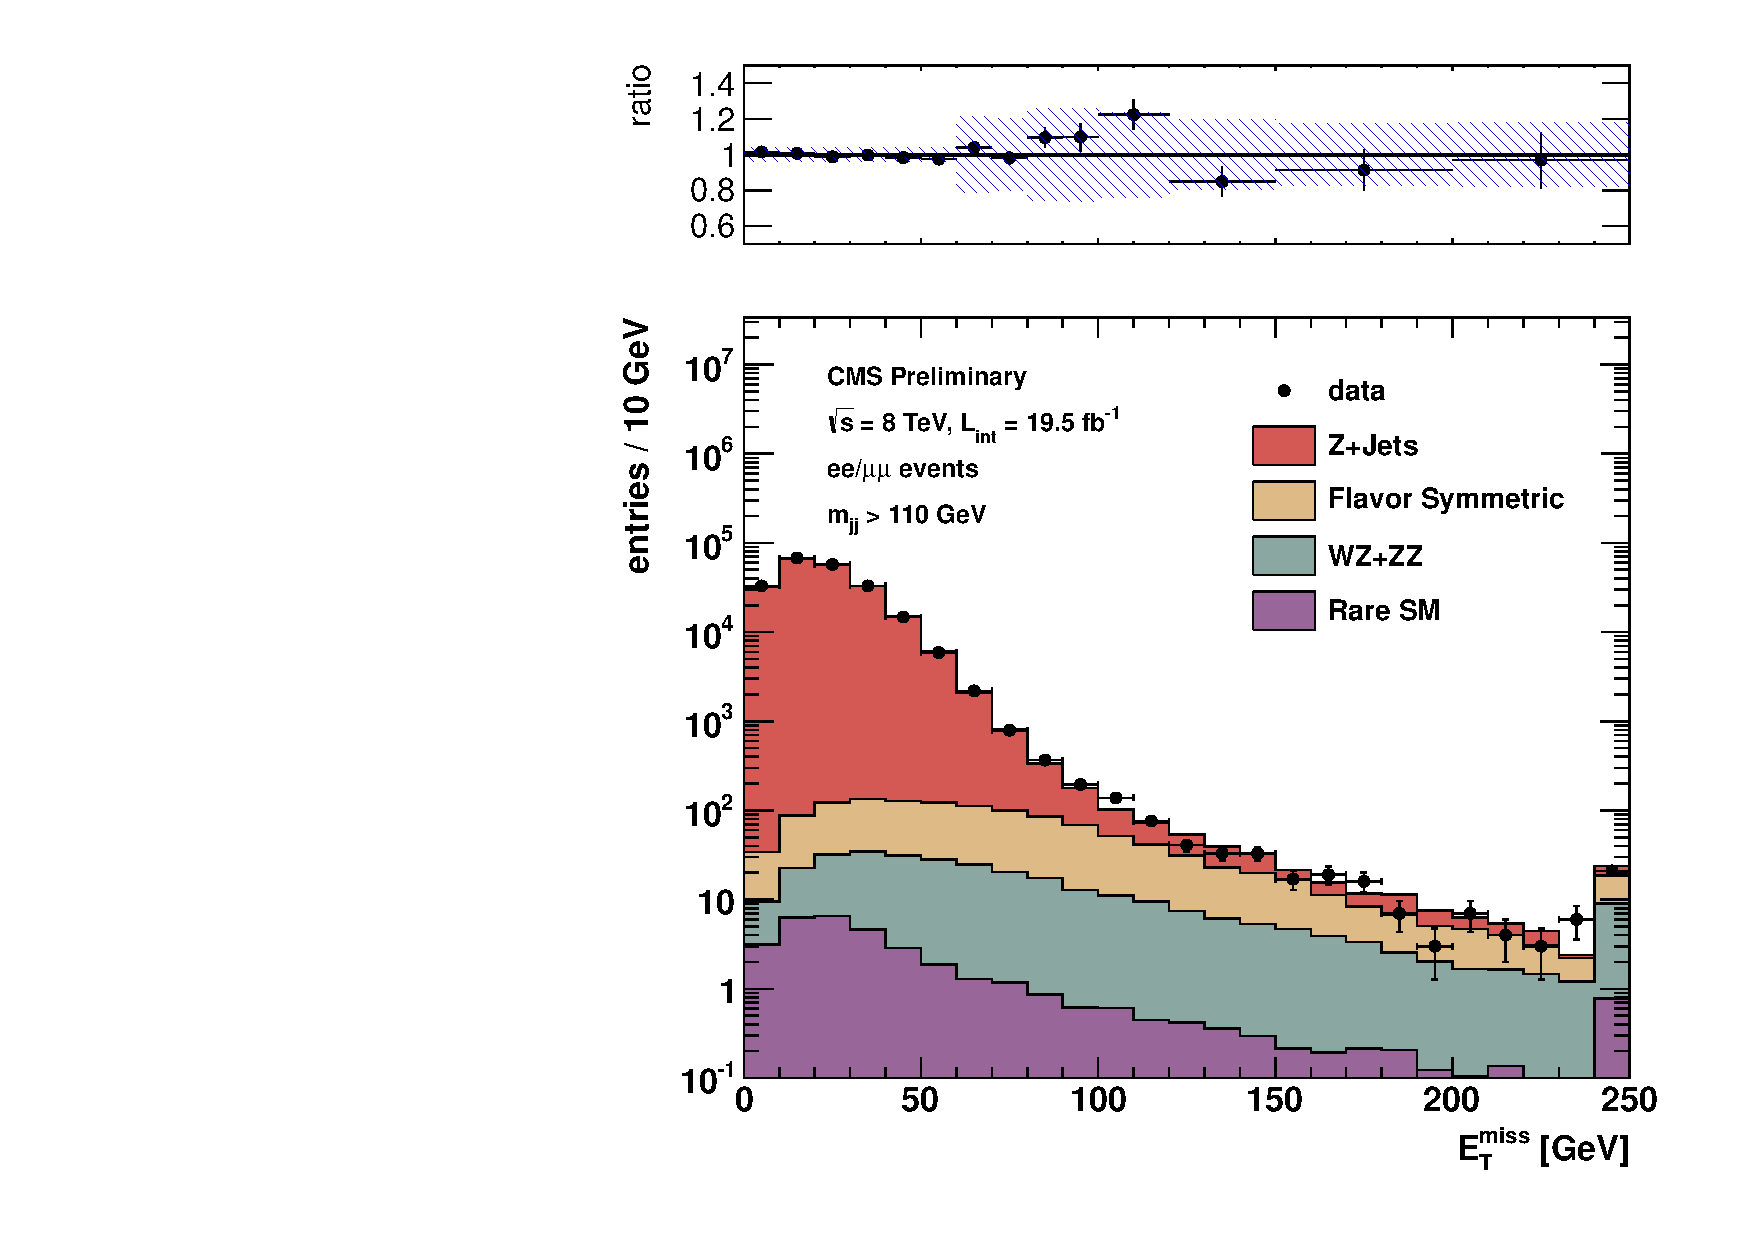
\includegraphics[width=0.49\textwidth]{plots/met_metall.pdf}
\end{tabular}
\caption{The \MET\ distribution after the dilepton mass requirement in the high dijet mass control region. The observed distribution in data
(black points) is compared with the sum of the predicted distributions from $\rm{Z}+\rm{jets}$, flavor-symmetric, sum of WZ and ZZ, and rare SM backgrounds. 
The ratio of observed to predicted yields in each bin is
indicated. The error bars indicate the statistical uncertainty in the data and the shaded band indicates the total background uncertainty.
\label{fig:results_targ_control}
}
\end{center}
\end{figure}

\begin{table}[htb]
\begin{center}
\footnotesize
\caption{\label{tab:results_targ_control}\footnotesize Summary of results in the targeted analysis, in the high dijet mass control region.
The total background is the sum of the \zjets\ background predicted from
the \MET\ templates method (\zjets\ bkg), the flavor-symmetric background predicted from e$\mu$ events (FS bkg), and the WZ and ZZ backgrounds predicted from MC
(WZ bkg and ZZ bkg). All uncertainties include both the statistical and systematic components. The Gaussian significance of the deviation between the data 
and total background is indicated for signal regions with at least 20 observed events. }
\begin{tabular}{l|c|c|c|c}


\hline
\hline
                      &   \MET\ 0--30 GeV   &  \MET\ 30--60 GeV   &  \MET\ 60--80 GeV   & \MET\ 80--100 GeV     \\

\hline

\hline
   \zjets\ bkg  & 157439.4 $\pm$ 6302.3 & 53676.6 $\pm$ 2151.8 & 2701.5 $\pm$ 595.1 & 358.7 $\pm$ 118.8   \\
         FS bkg & 180.2 $\pm$ 30.1 & 290.8 $\pm$ 48.4 & 167.2 $\pm$ 28.0 & 123.8 $\pm$ 20.8   \\
         WZ bkg & 41.6 $\pm$ 20.8 & 69.9 $\pm$ 35.0 & 33.4 $\pm$ 16.7 &  21.0 $\pm$ 10.5   \\
         ZZ bkg &   6.6 $\pm$ 3.3 &  14.8 $\pm$ 7.4 &   9.4 $\pm$ 4.7 &    7.8 $\pm$ 3.9   \\
    Rare SM bkg &  16.0 $\pm$ 8.0 &   9.4 $\pm$ 4.7 &   2.5 $\pm$ 1.2 &    1.5 $\pm$ 0.7   \\

\hline

      Total bkg & 157683.7 $\pm$ 6302.4 & 54061.4 $\pm$ 2152.6 & 2914.0 $\pm$ 596.0 & 512.8 $\pm$ 121.2   \\

           Data &          158074 &           53608 &            2983 &               562  \\
\hline
\hline
                      &\MET\ 100--120 GeV   &\MET\ 120--150 GeV   &\MET\ 150--200 GeV   & \MET\ $>$ 200 GeV  \\
\hline
\hline

\zjets\ bkg & 81.7 $\pm$ 27.3 & 52.0 $\pm$ 17.9 &  20.0 $\pm$ 6.9 &    9.5 $\pm$ 3.4   \\
         FS bkg & 72.5 $\pm$ 12.3 & 55.1 $\pm$ 13.4 & 31.4 $\pm$ 12.4 &   15.9 $\pm$ 6.3   \\
         WZ bkg &  13.6 $\pm$ 6.8 &  11.6 $\pm$ 5.8 &   9.7 $\pm$ 4.9 &    7.2 $\pm$ 3.6   \\
         ZZ bkg &   6.0 $\pm$ 3.0 &   6.2 $\pm$ 3.1 &   5.9 $\pm$ 3.0 &    5.6 $\pm$ 2.8   \\
    Rare SM bkg &   1.1 $\pm$ 0.5 &   1.1 $\pm$ 0.5 &   0.9 $\pm$ 0.5 &    1.1 $\pm$ 0.5   \\
\hline
      Total bkg & 174.9 $\pm$ 30.9 & 126.0 $\pm$ 23.3 & 67.9 $\pm$ 15.3 &   39.2 $\pm$ 8.5   \\
           Data &             214 &             107 &              62 &                38  \\
\hline
\hline

\end{tabular}
\end{center}
\end{table}

\clearpage

\begin{figure}[!h]
\begin{center}
\begin{tabular}{cc}
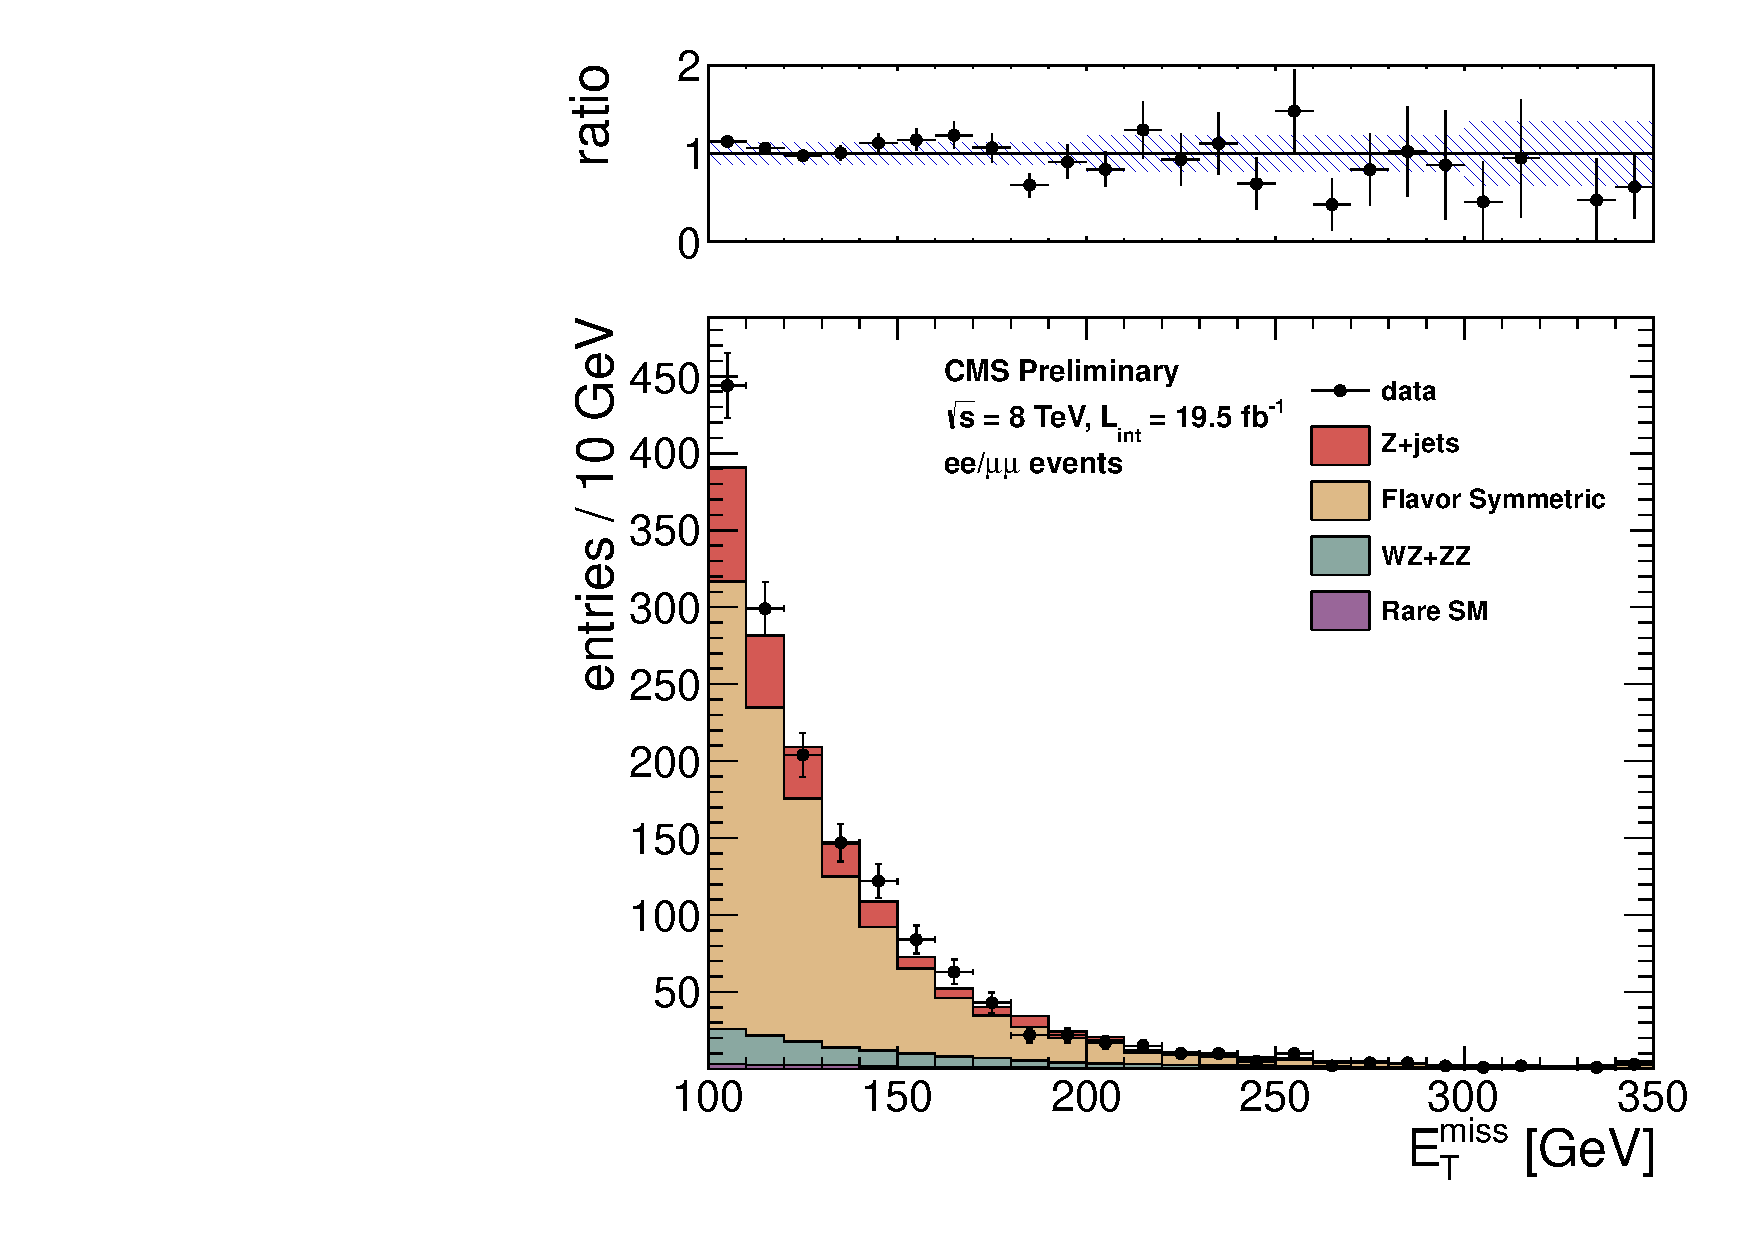
\includegraphics[width=0.6\textwidth]{plots/pfmet_all_19p5fb_zoom100.pdf}
\end{tabular}
\caption{ Results for the inclusive analysis, the same as Fig.~\ref{fig:results_incl} but zoomed in on the signal region \MET\ $>$ 100 GeV and on linear scale.
\label{fig:results_incl_zoom}
}
\end{center}
\end{figure}

\begin{figure}[!h]
\begin{center}
\begin{tabular}{cc}
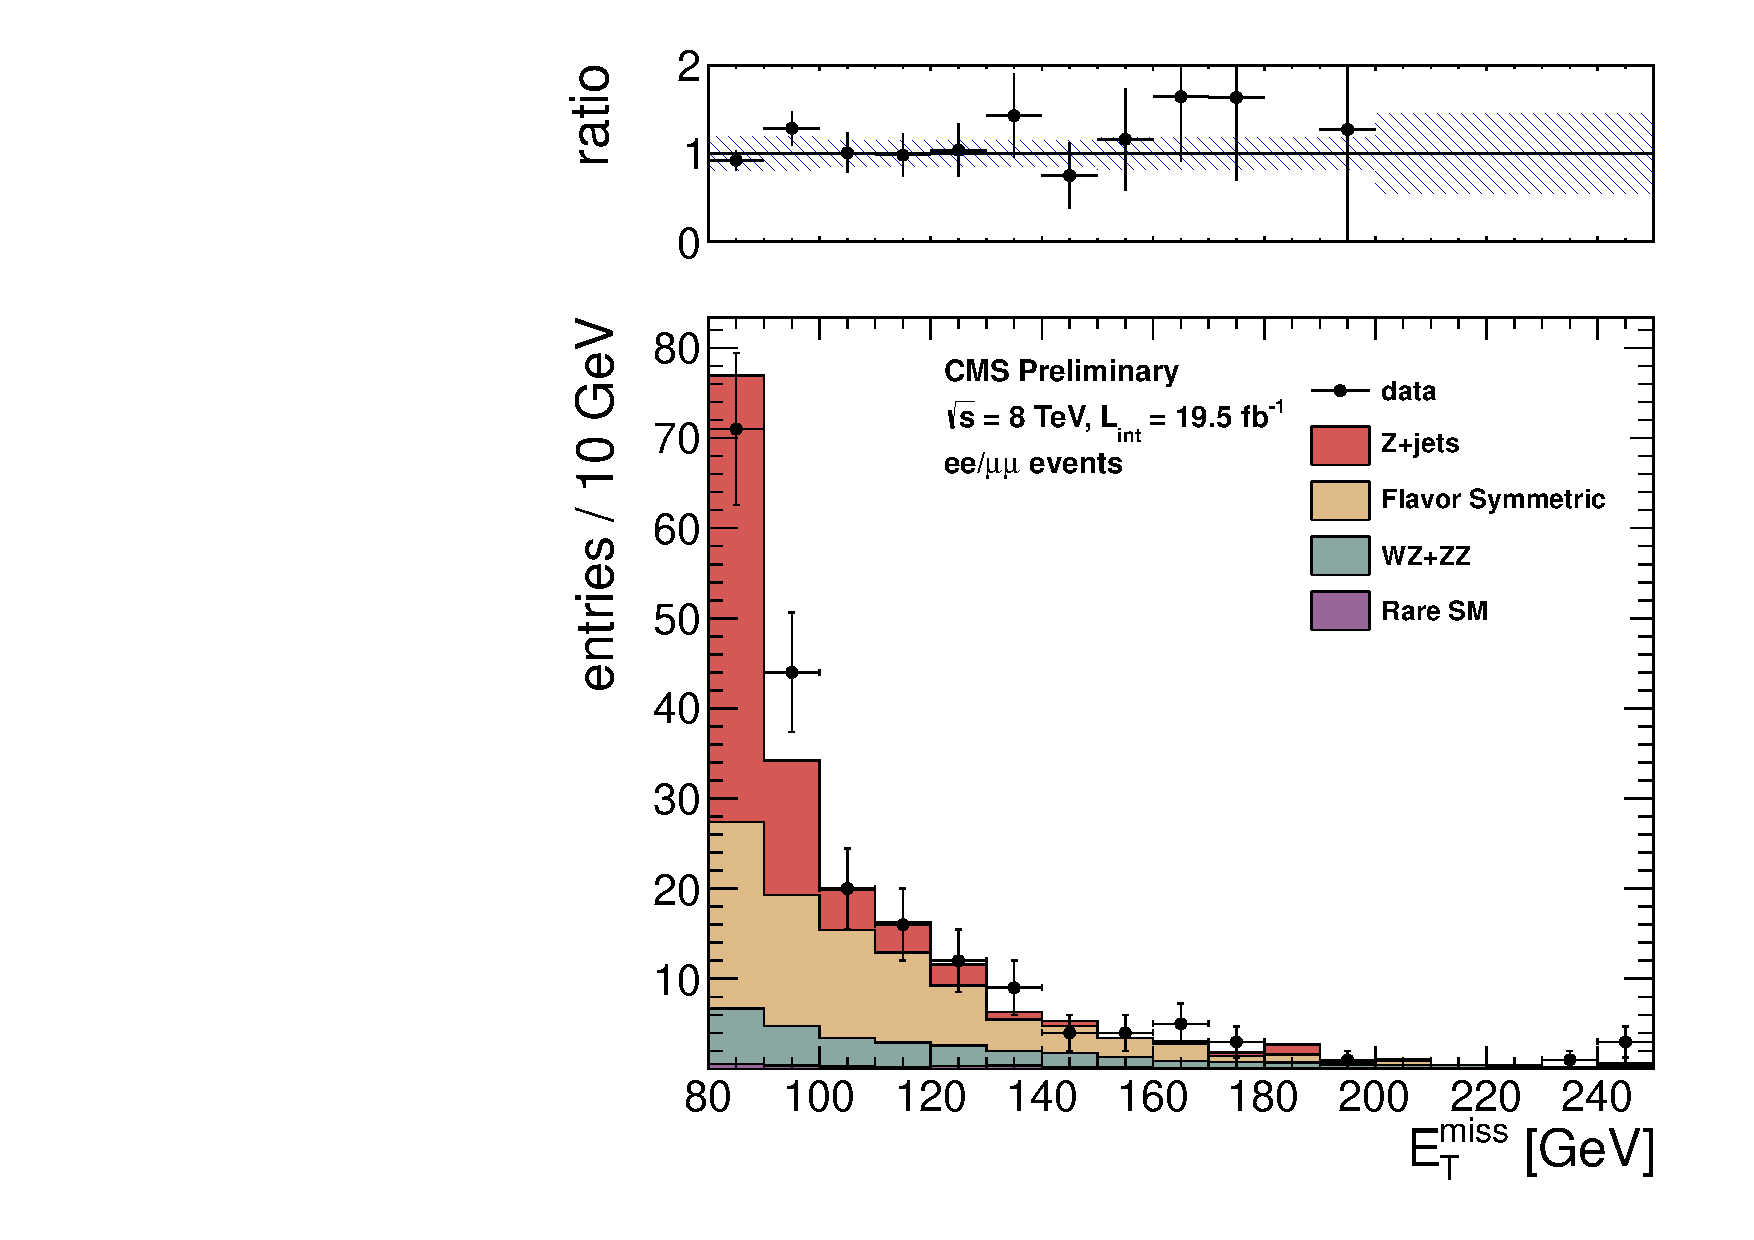
\includegraphics[width=0.6\textwidth]{plots/pfmet_bveto_all_19p5fb_zoom80.pdf}
\end{tabular}
\caption{ Results for the targeted analysis, the same as Fig.~\ref{fig:results_targ} but zoomed in on the signal region \MET\ $>$ 80 GeV and on linear scale.
\label{fig:results_targ_zoom}
}
\end{center}
\end{figure}

\clearpage
